\documentclass[12pt]{article}
\usepackage{amsfonts, amssymb, amsmath, amsthm}
\usepackage[margin=1in]{geometry}
\usepackage{tikz}
\usetikzlibrary{patterns, decorations.pathreplacing}

\pagestyle{myheadings}
\markright{Explainer: Rudin 4.15 --- Open Maps are Monotonic\hfill}

\newcommand{\R}{\mathbb{R}}

\begin{document}

\begin{center}
    \textbf{\Large Continuous Open Maps $\R \to \R$ are Monotonic}\\[0.5em]
    \large A visual guide to Rudin 4.15
\end{center}

\section{What is an Open Map?}

A map $f: X \to Y$ is \textbf{open} if it sends open sets to open sets:
\[
V \text{ open in } X \implies f(V) \text{ open in } Y
\]

\begin{center}
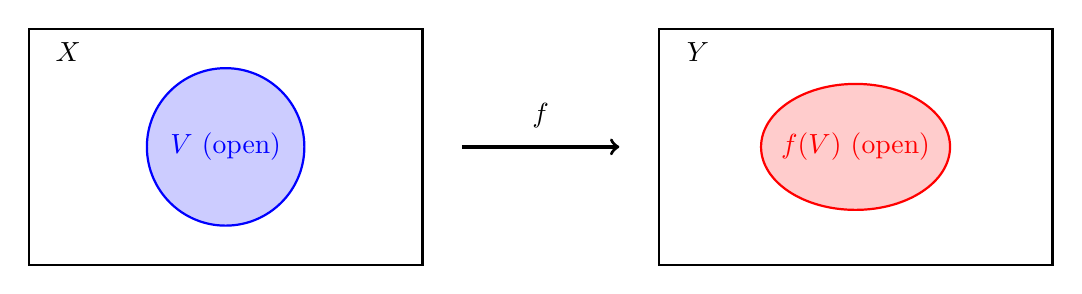
\begin{tikzpicture}[scale=1]
    % Domain
    \begin{scope}[xshift=-4cm]
        \draw[thick] (-2.5, -1.5) rectangle (2.5, 1.5);
        \node at (-2, 1.2) {$X$};
        \draw[blue, thick, fill=blue!20] (0, 0) circle (1);
        \node[blue] at (0, 0) {$V$ (open)};
    \end{scope}

    \draw[->, very thick] (-1, 0) -- (1, 0);
    \node at (0, 0.4) {$f$};

    % Codomain
    \begin{scope}[xshift=4cm]
        \draw[thick] (-2.5, -1.5) rectangle (2.5, 1.5);
        \node at (-2, 1.2) {$Y$};
        \draw[red, thick, fill=red!20] (0, 0) ellipse (1.2 and 0.8);
        \node[red] at (0, 0) {$f(V)$ (open)};
    \end{scope}
\end{tikzpicture}
\end{center}

\textbf{Note:} This is \emph{not} the same as continuity! Continuity means \emph{preimages} of open sets are open. An open map means \emph{images} of open sets are open.

\section{What Does Monotonic Mean?}

$f$ is \textbf{monotonic} if it is either entirely increasing or entirely decreasing:

\begin{center}
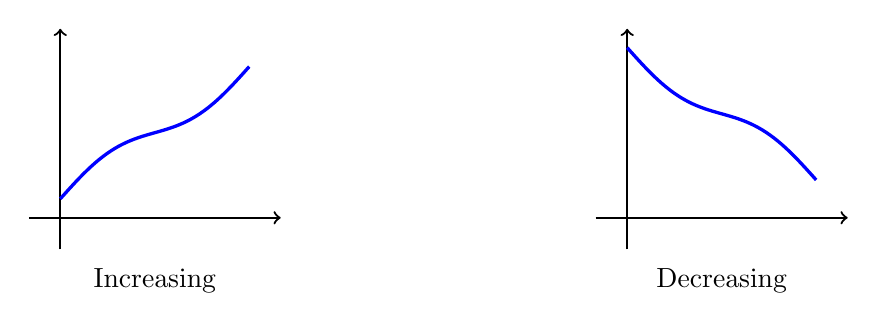
\begin{tikzpicture}[scale=0.8]
    % Increasing
    \begin{scope}[xshift=-4.5cm]
        \draw[thick, ->] (-0.5, 0) -- (3.5, 0);
        \draw[thick, ->] (0, -0.5) -- (0, 3);
        \draw[blue, very thick, domain=0:3, samples=50] plot (\x, {0.3 + 0.7*\x + 0.2*sin(120*\x)});
        \node at (1.5, -1) {Increasing};
    \end{scope}

    % Decreasing
    \begin{scope}[xshift=4.5cm]
        \draw[thick, ->] (-0.5, 0) -- (3.5, 0);
        \draw[thick, ->] (0, -0.5) -- (0, 3);
        \draw[blue, very thick, domain=0:3, samples=50] plot (\x, {2.7 - 0.7*\x - 0.2*sin(120*\x)});
        \node at (1.5, -1) {Decreasing};
    \end{scope}
\end{tikzpicture}
\end{center}

\section{The Claim}

\begin{center}
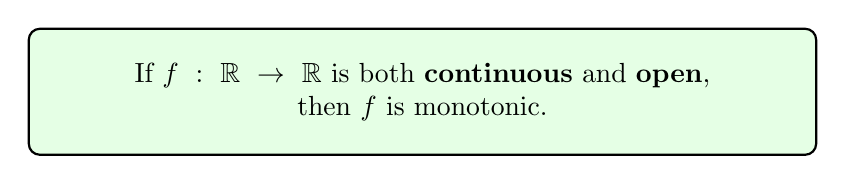
\begin{tikzpicture}
    \draw[thick, rounded corners, fill=green!10] (-5, -0.8) rectangle (5, 0.8);
    \node[text width=9cm, align=center] at (0, 0) {
        If $f: \R \to \R$ is both \textbf{continuous} and \textbf{open},\\
        then $f$ is monotonic.
    };
\end{tikzpicture}
\end{center}

\section{Key Insight: Local Extrema Kill Openness}

If $f$ is not monotonic, it must have a \textbf{local maximum} or \textbf{local minimum}.

\begin{center}
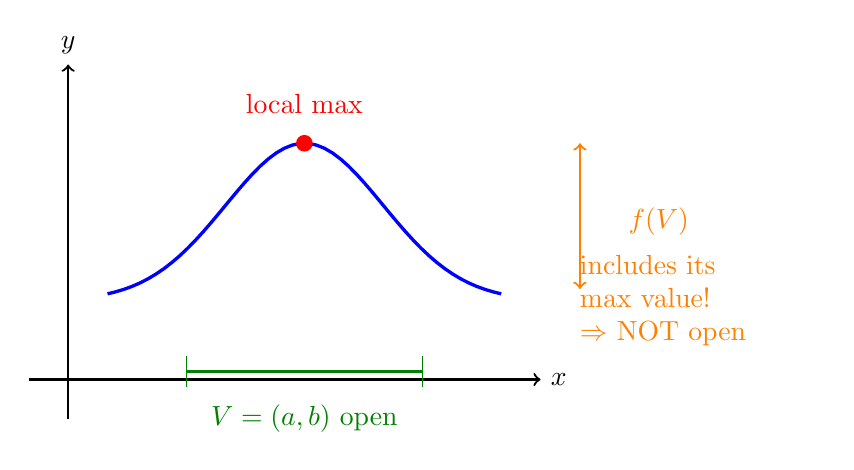
\begin{tikzpicture}[scale=1]
    \draw[thick, ->] (-0.5, 0) -- (6, 0) node[right] {$x$};
    \draw[thick, ->] (0, -0.5) -- (0, 4) node[above] {$y$};

    % Function with a local max
    \draw[blue, very thick, domain=0.5:5.5, samples=50] plot (\x, {1 + 2*exp(-(\x - 3)*(\x - 3)/2)});

    % Local max
    \fill[red] (3, 3) circle (3pt);
    \node[red] at (3, 3.5) {local max};

    % Open interval around max
    \draw[green!50!black, very thick] (1.5, 0.1) -- (4.5, 0.1);
    \draw[green!50!black] (1.5, -0.1) -- (1.5, 0.3);
    \draw[green!50!black] (4.5, -0.1) -- (4.5, 0.3);
    \node[green!50!black] at (3, -0.5) {$V = (a, b)$ open};

    % Image of V
    \draw[<->, orange, thick] (6.5, 1.15) -- (6.5, 3);
    \node[orange] at (7.5, 2) {$f(V)$};
    \node[orange, text width=3cm, align=left] at (8, 1) {includes its\\max value!\\$\Rightarrow$ NOT open};
\end{tikzpicture}
\end{center}

\subsection{Why the Image Isn't Open}

\begin{center}
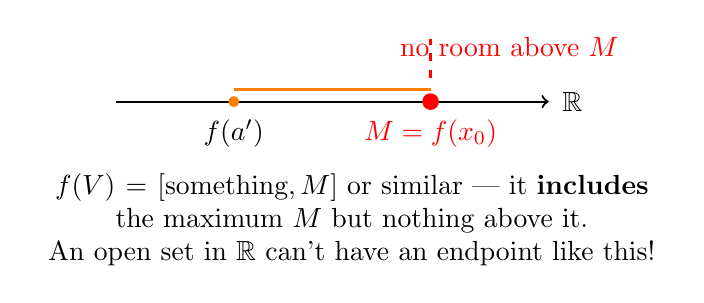
\begin{tikzpicture}[scale=1]
    % The image on the y-axis
    \draw[thick, ->] (-0.5, 0) -- (5, 0);
    \node at (5.3, 0) {$\R$};

    % f(V) as an interval
    \draw[orange, very thick] (1, 0.15) -- (3.5, 0.15);
    \fill[orange] (1, 0) circle (2pt);
    \fill[red] (3.5, 0) circle (3pt);

    \node at (1, -0.4) {$f(a')$};
    \node[red] at (3.5, -0.4) {$M = f(x_0)$};

    % Explanation
    \node[text width=8cm, align=center] at (2.5, -1.5) {
        $f(V) = [\text{something}, M]$ or similar --- it \textbf{includes}\\
        the maximum $M$ but nothing above it.\\
        An open set in $\R$ can't have an endpoint like this!
    };

    % Detail
    \draw[red, thick, dashed] (3.5, 0.3) -- (3.5, 0.8);
    \node[red] at (4.5, 0.7) {no room above $M$};
\end{tikzpicture}
\end{center}

\section{The Contrapositive Argument}

\begin{center}
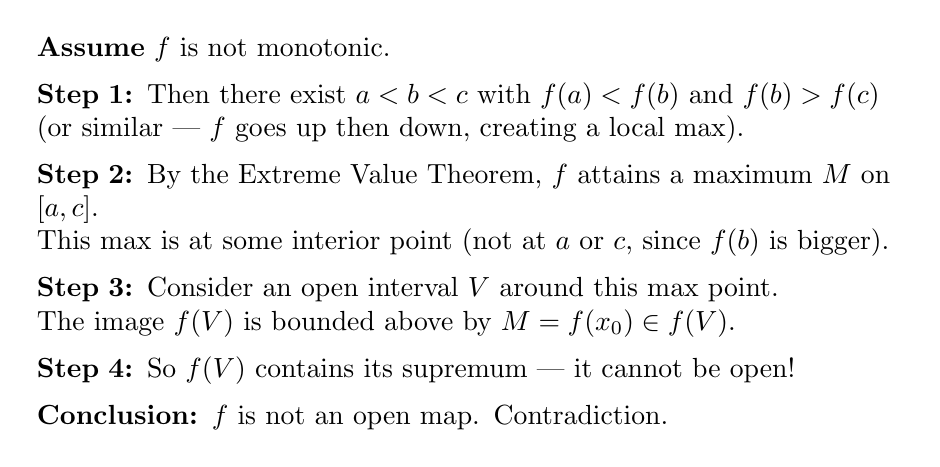
\begin{tikzpicture}[scale=1]
    \node[text width=11cm, align=left] at (0, 0) {
        \textbf{Assume} $f$ is not monotonic.\\[0.5em]
        \textbf{Step 1:} Then there exist $a < b < c$ with $f(a) < f(b)$ and $f(b) > f(c)$\\
        (or similar --- $f$ goes up then down, creating a local max).\\[0.5em]
        \textbf{Step 2:} By the Extreme Value Theorem, $f$ attains a maximum $M$ on $[a, c]$.\\
        This max is at some interior point (not at $a$ or $c$, since $f(b)$ is bigger).\\[0.5em]
        \textbf{Step 3:} Consider an open interval $V$ around this max point.\\
        The image $f(V)$ is bounded above by $M = f(x_0) \in f(V)$.\\[0.5em]
        \textbf{Step 4:} So $f(V)$ contains its supremum --- it cannot be open!\\[0.5em]
        \textbf{Conclusion:} $f$ is not an open map. Contradiction.
    };
\end{tikzpicture}
\end{center}

\section{Examples}

\begin{center}
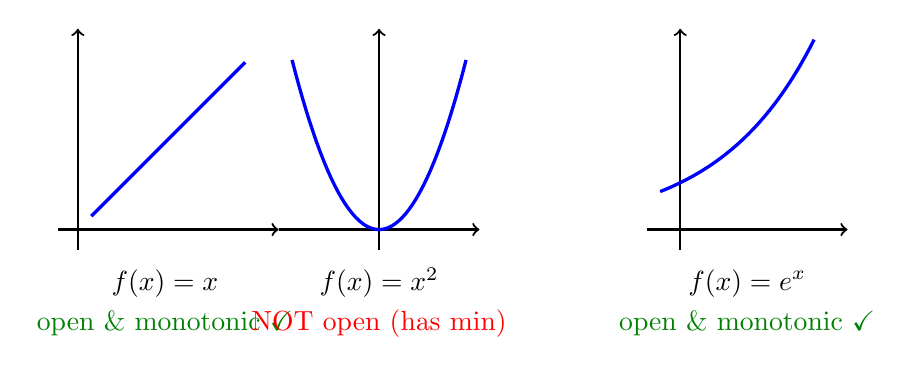
\begin{tikzpicture}[scale=0.85]
    % f(x) = x: open and monotonic
    \begin{scope}[xshift=-4.5cm]
        \draw[thick, ->] (-0.3, 0) -- (3, 0);
        \draw[thick, ->] (0, -0.3) -- (0, 3);
        \draw[blue, very thick] (0.2, 0.2) -- (2.5, 2.5);
        \node at (1.3, -0.8) {$f(x) = x$};
        \node[green!50!black] at (1.3, -1.4) {open \& monotonic \checkmark};
    \end{scope}

    % f(x) = x^2: not open (has a min)
    \begin{scope}[xshift=0cm]
        \draw[thick, ->] (-1.5, 0) -- (1.5, 0);
        \draw[thick, ->] (0, -0.3) -- (0, 3);
        \draw[blue, very thick, domain=-1.3:1.3, samples=50] plot (\x, {1.5*\x*\x});
        \node at (0, -0.8) {$f(x) = x^2$};
        \node[red] at (0, -1.4) {NOT open (has min)};
    \end{scope}

    % f(x) = e^x: open and monotonic
    \begin{scope}[xshift=4.5cm]
        \draw[thick, ->] (-0.5, 0) -- (2.5, 0);
        \draw[thick, ->] (0, -0.3) -- (0, 3);
        \draw[blue, very thick, domain=-0.3:2, samples=50] plot (\x, {0.7*exp(0.7*\x)});
        \node at (1, -0.8) {$f(x) = e^x$};
        \node[green!50!black] at (1, -1.4) {open \& monotonic \checkmark};
    \end{scope}
\end{tikzpicture}
\end{center}

\end{document}
